\chapter{Diseño de la propuesta}

En este capítulo vamos a analizar los requisitos de nuestra red y a establecer una propuesta de diseño físico para la misma. Además vamos a caracterizar los distintos nodos que compondrán nuestra red.

Vamos a partir del plano de nuestra oficina en la que queremos montar la red. Como aproximación vamos a suponer que se trata de una nueva oficina de la Universidad de Granada en la que van a encontrarse 5 trabajadores, cada uno de ellos con sus respectivos puestos de trabajo. La planta de la oficina sería la mostrada en la figura \ref{fig:planta_oficina}:

\begin{figure}[!h]
    \centering
    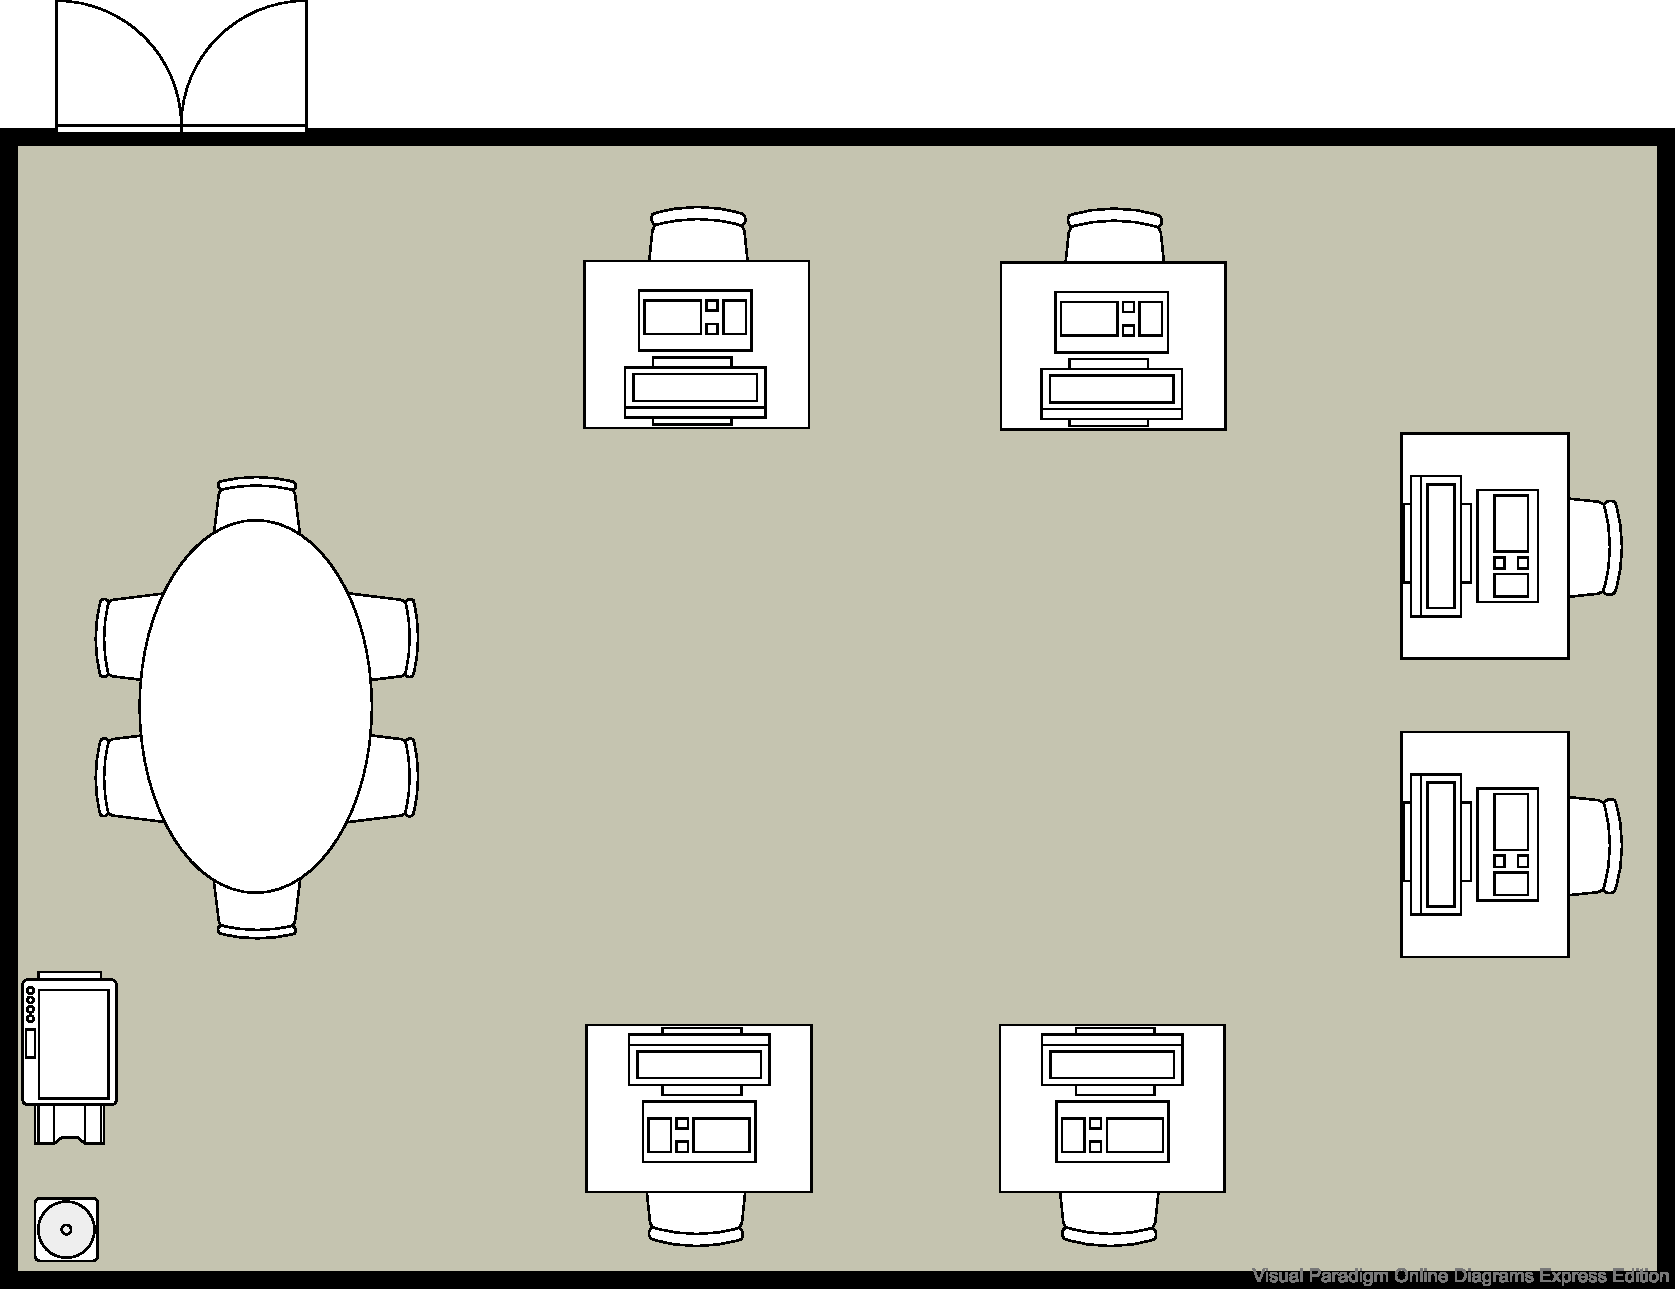
\includegraphics[width=\textwidth]{imagenes/figuras/Plano oficina.pdf}
    \caption{Planta de la oficina en la que vamos a montar nuestra red.}
    \label{fig:planta_oficina}
\end{figure}

A partir de este plano vamos a identificar los requisitos que debe cumplir nuestra red y vamos a hacer un diseño base para la misma. Además veremos como no tenemos que decidir exactamente cuantos equipos finales habrá en la misma ni a donde van conectados, pues la red será capaz de detectarlos automáticamente y configurarlos según su tipo.

\section{Requisitos de una red corporativa}

Empezaremos describiendo el entorno en el que nos encontramos y obteniendo los distintos requisitos funcionales de la red, para luego identificar los tipos de nodo que se han de conectar así como las tareas que deben desempeñar los usuarios finales para utilizar nuestra red.

\subsection{Descripción del entorno y análisis de requisitos}

En esta propuesta nos encontramos en una oficina con puestos informáticos, teléfonos VoIP y una impresora compartida. Además sabemos que se quiere instalar una red de videovigilancia en la oficina para controlar la seguridad. Queremos diseñar una red que sea eficiente en rendimiento y coste a la vez que sea segura y, automáticamente se pueda ampliar tanto como se necesite (así como instalar redes similares en múltiples oficinas).

Formalmente la lista de requisitos funcionales de la red es la siguiente:

\begin{itemize}
    \item La red debe estar operativa las 24 horas del día, 7 días a la semana (24x7).
    \item Solo se instalará un único cableado para los distintos dispositivos, es decir, la las mismas líneas de datos transportarán datos de las cámaras de seguridad, los teléfonos, los ordenadores y cualquier otro dispositivo que se pueda (quiera) conectar.
    \item Se incluirá acceso mediante red WiFi para los dispositivos de los trabajadores y los posibles clientes.
    \item Deberá poderse ampliar la red sin tener que instalar una nueva, simplemente añadiendo los dispositivos necesarios sin tener que tocar ninguno de los existentes.
    \item Los usuarios no son expertos en tecnologías, por lo que debe una ser red fiable que no les ocasione molestias a la hora de trabajar.
    \item La red se debe poder administrar remotamente, para evitar desplazamientos de técnicos a la oficina.
    \item Los usuarios no deben poder conectarse a la red de seguridad desde sus dispositivos (ordenadores de trabajo o dispositivos WiFi). Si deben poder conectarse entre ellos y al servidor de contenido sobre el que trabajan.
    \item Los usuarios podrán utilizar recursos compartidos como la impresora de red.
    \item La red deberá ser tolerante a fallos.
\end{itemize}

Ahora vamos a caracterizar los distintos elementos que conforman nuestra red antes de hacer el diseño.

\subsection{Tipos de nodos}

A nuestra red deberán conectarse: ordenadores de los trabajadores (puestos fijos), teléfonos VoIP, cámaras de seguridad, impresoras en red y dispositivos inalámbricos. Cada uno de los tipos de nodos tienen unos requisitos distintos: de esta forma los teléfonos tienen la necesidad de enviar y recibir paquetes con la menor latencia posible (aunque permiten que se pierdan algunos paquetes); las cámaras de seguridad admiten paquetes con latencia alta y pérdida de paquetes, pero tienen un requisito de ancho de banda constante al estar continuamente enviando vídeo al servidor de seguridad para su grabación. Los ordenadores y la impresora no tienen requisitos de velocidad (siempre que ofrezcan un rendimiento suficiente que no empeore la calidad de la experiencia de los trabajadores, es decir, que no sea tan lenta que los usuarios desesperen) pero admiten que se pierdan paquetes de datos.

\subsection{Usuarios finales}

Los usuarios finales de la red son los trabajadores de la oficina y los clientes o colaboradores que traigan sus propios dispositivos y necesiten una conexión de red. Estos usuarios no deben tener consciencia de la red desde un punto de vista técnico. Su mayor relación con la red será introducir la clave de acceso a la red inalámbrica en sus dispositivos, nada más.

\subsection{Tareas de administración}

Las tareas de administración sobre la red tendrán que ser mínimas, siendo la principal el cambio de la clave de acceso de la red inalámbrica. Cuando sea necesario instalar un nuevo dispositivo, el administrador solo deberá encargarse de conectarlo a la red, y esta última será la encargada de configurar de forma automática todos los parámetros del nuevo dispositivo (Dirección IP, puerto de acceso, permisos de acceso a otros dispositivos, etc.).

\section{Diseño físico de la red.}

Vamos a realizar el planteamiento físico de la red sobre el plano de planta de la oficina expuesto anteriormente. En la figura \ref{fig:diseño_fisico} vemos como queda planteado el diseño física. Ahora vamos a discutir algunas cuestiones de diseño para entender como llegamos hasta él.

En primer lugar está la decisión de cuantos switches poner, en este caso hemos optado por 3 switches ethernet y un punto de acceso inalámbrico. Otra opción sería poner un único switch grande pero por razones de costo (un switch grande compatible con OpenFlow es mucho más caro que varios más pequeños también compatibles) se ha decidido la opción de múltiples switches. Luego está la topología a usar. Cisco recomienda en sus diseños utilizar topologías en árbol, donde los switches de acceso (a los que se conectan los usuarios finales) se conectan entre sí a otros swiches de niveles superiores \cite{cisco:10.5555/975411}. Sin embargo nosotros hemos elegido empezar con una topología en malla donde los switches están interconectados entre sí. Esta configuración nos permite tener una mayor redundancia en caso de caída de enlaces y nos permitirá, en caso que sea necesario, ejecutar aplicaciones de enlaces redundantes en el controlador SDN si necesitáramos mayor ancho de banda en la red, sin tener que cambiar las conexiones existentes. Esta topología nos permite ampliar la red de forma sencilla asegurando la redundancia. La topología en malla introduce un problema que tendremos que resolver: la aparición de bucles en la red. Estos bucles pueden ser eliminados de la topología lógica de la red utilizando el protocolo \acrshort{stp}, \acrlong{stp}, que detecta los bucles en la red y deshabilita los puertos que lo causan, volviéndolos a activar en caso que sean necesarios (caída, sobrecarga, agrupamiento de enlaces, etc). Además podemos ver que en nuestro diseño no existen capas diferenciadas entre switches de acceso y de distribución, sino que todos los switches son de acceso (donde se conectan los usuarios finales). De este modo no estamos introduciendo en la red más dispositivos que mantener y que, principalmente, comprar.

\begin{figure}[!h]
    \centering
    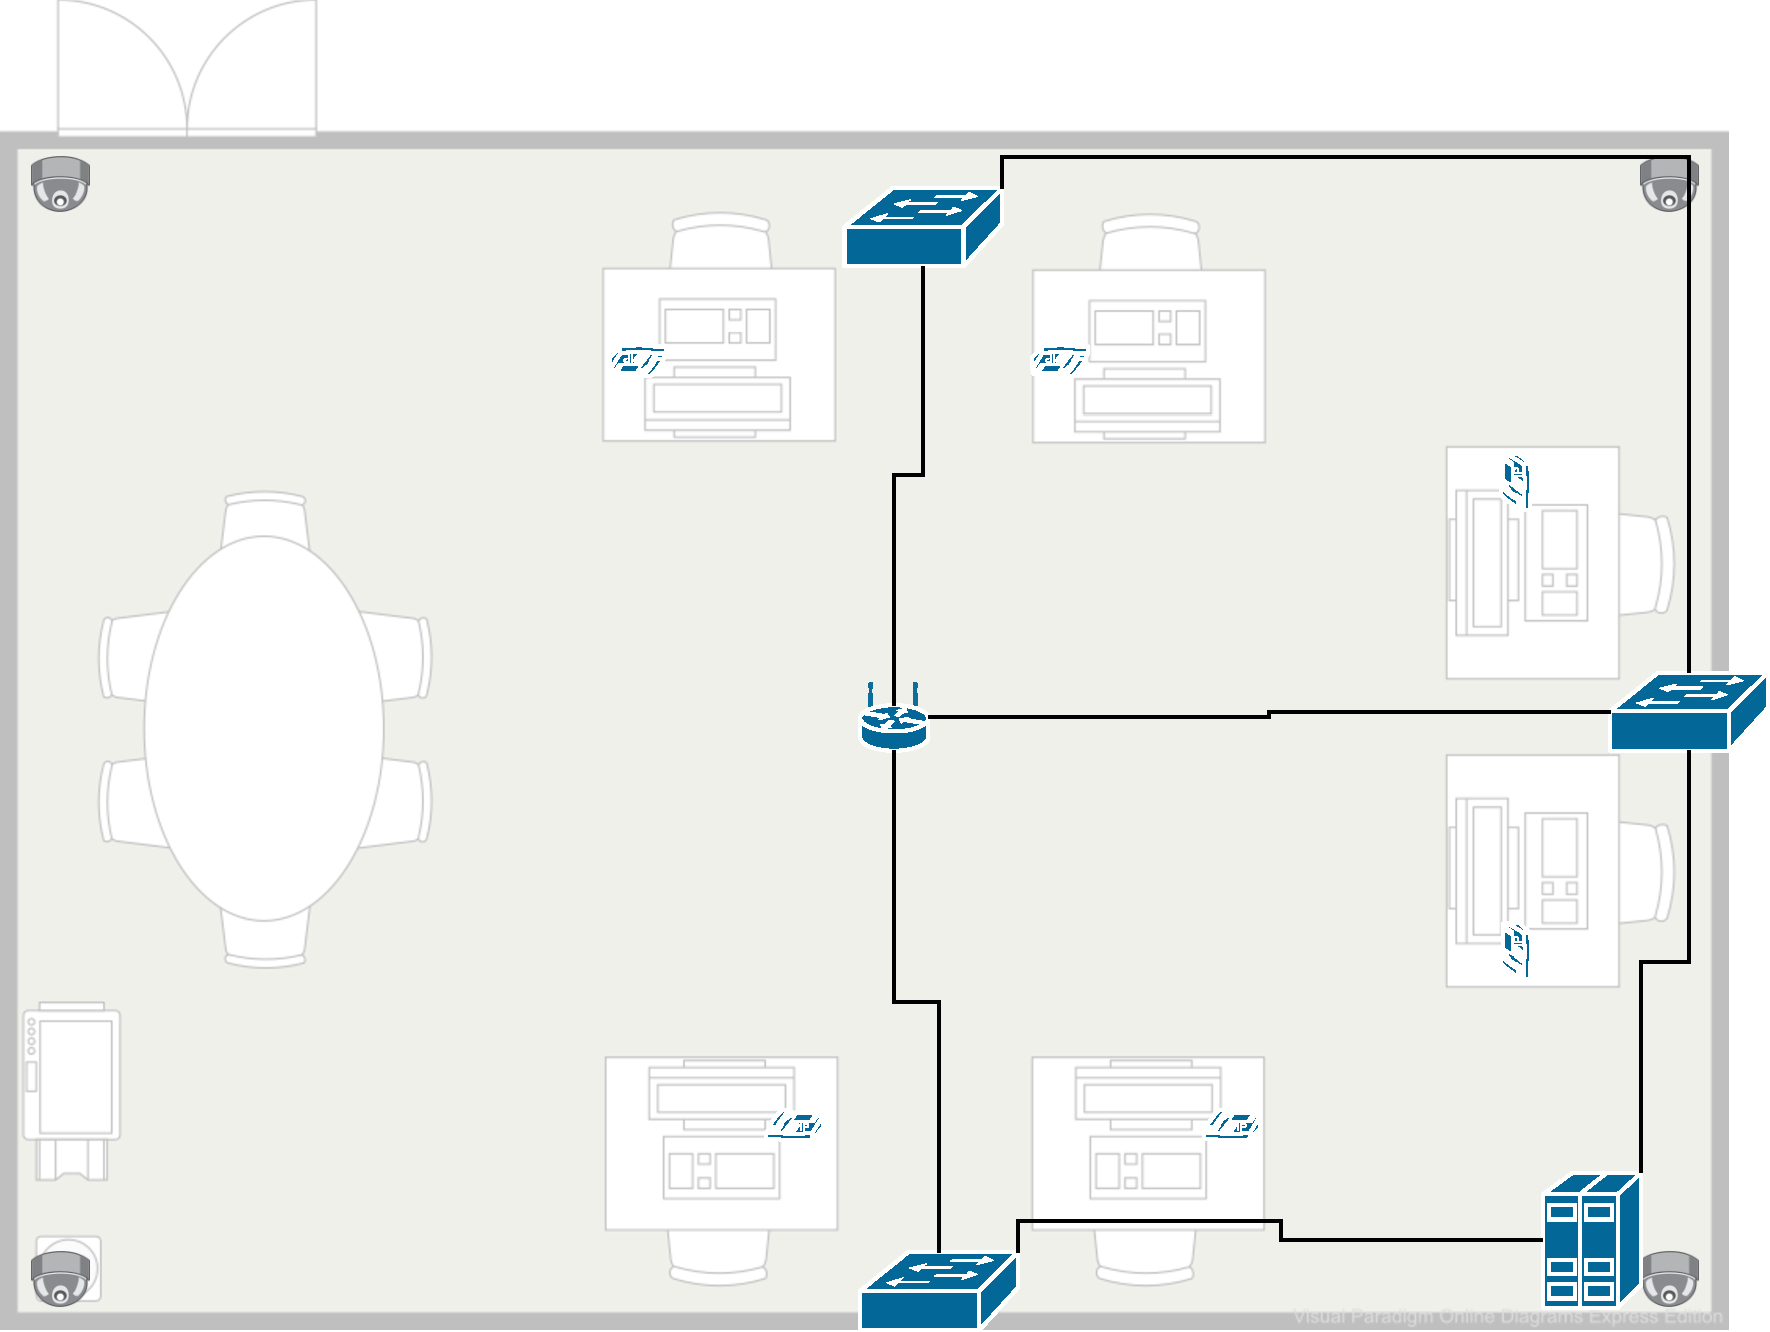
\includegraphics[width=\textwidth]{imagenes/figuras/requisitos_red_con_plano.pdf}
    \caption{Diseño físico de la red.}
    \label{fig:diseño_fisico}
\end{figure}

\section{Diseño lógico de la red.}

Una vez tenemos el diseño físico de la red (los dispositivos propiamente dichos) vamos a encargarnos del diseño lógico, es decir, como tiene que estar configurada la red para funcionar correctamente y cumplir los requisitos que hemos identificado anteriormente.

Un punto vital a tener en cuenta en este apartado es que estamos diseñando una red definida por software, con todas las ventajas que ello conlleva, por lo que tenemos que pensar en como solucionar los problemas de una forma abstracta y general, pues el controlador (la aplicación que genera las tablas de encaminamiento de los switches) es el mismo para todos los switches de la red, por lo que tendremos que pensar en la red completa como un todo y no pensar cosas como \emph{''Pues este switch que está cerca de la impresora lo configuro de una manera y el de la otra esquina de la sala, de otra manera completamente diferente''} ya que esa forma de diseñar redes conlleva problemas de mantenimiento (configuración separada de cada dispositivo de red) y no estaríamos aprovechando la capacidad que nos brindan las SDN de tratar la red como un proyecto software que podemos modificar y optimizar de forma incremental para resolver los problemas que nos puedan surgir. Recordemos que en una red tradicional una vez compras un equipo específico no nos podemos salir de las características que trae de fábrica, en una SDN podemos instalar y ejecutar tantas funcionalidades como aplicaciones desarrollemos.

Tenemos que separar los dispositivos en distintas subredes, de forma que diferenciemos los distintos servicios y no puedan verse entre ellos. Si solo hiciéramos esta distinción usando distintas redes IP los dispositivos podrían seguir comunicándose si así se quisiera (posible ataque a la red) ya que seguirían conectados a la misma red ethernet de área local (aunque sus direcciones IP no estuvieran en la misma subred). Por esto vamos a dividir la red en 3 \acrshort{vlan}\footnote{\acrlong{vlan}, redes LAN que funcionan en una misma infraestructura de red pero que lógicamente, son independientes entre si} distintas: Seguridad, telefonía y acceso general. Para lograr esta separación tenemos que encontrar alguna manera de asignar a cada dispositivo una VLAN distinta de forma automática, para mantener así la característica autoconfigurable de la red. Esta es una tarea que podemos lograr fácilmente mediante una aplicación de Ryu que asigne a cada puerto de cada switch una VLAN distinta.

Además necesitamos disponer de uno o varios servidores que ejecuten los servicios necesarios (ruteo de paquetes hacia internet, servidor de videovigilancia, servidor de telefonía e incluso el propio controlador de la red, entre otros servicios que pueden surgir más adelante). Este servidor tiene que ser accesible por todos los dispositivos, por lo que tendrá (o tendrán) que ser parte de todas las VLAN. 

Con esta información podemos generar un esquema lógico de la red que estamos diseñando. Este esquema es la figura \ref{fig:diseño_logico}.

\begin{figure}[!h]
    \centering
    \includegraphics[width=\textwidth]{imagenes/figuras/diseño_logico.pdf}
    \caption{Diseño lógico de la red.}
    \label{fig:diseño_logico}
\end{figure}

Aquí podemos ver las distintas VLAN y como están interconectados los distintos equipos de la red. En color rojo tenemos los enlaces pertenecientes a la VLAN de acceso general, en verde tenemos los enlaces de la VLAN de seguridad y en azul tenemos los enlaces pertenecientes a la red virtual de telefonía. Además en negro tenemos los enlaces \emph{trunk}, es decir, los enlaces que llevan paquetes de múltiples VLANs.


\section{Implementación de la red en un entorno virtualizado}

Una vez que hemos analizado los requisitos de nuestra red y terminado el diseño lógico de la red podemos simular dicho escenario en un laboratorio de pruebas virtual para poder hacer pruebas 

\subsection{Diseño general en MiniEdit}
Vamos a empezar haciendo un esquema básico de la red utilizando el editor gráfico de Mininet: MiniEdit

Cabe destacar que, debido a capacidad limitada de procesamiento vamos a limitar la maqueta de la red a solo dos dispositivos de cada tipo. Como podemos ver en la Figura \ref{fig:miniedit} MiniEdit nos permite crear un armazón de la red que luego podremos modificar libremente. Esto es debido a que MiniEdit permite exportar un script Python que ejecuta la red. Este script puede ser modificado para ajustar parámetros de los nodos de red que no están disponibles desde la interfaz gráfica.

\begin{figure}[!h]
    \centering
    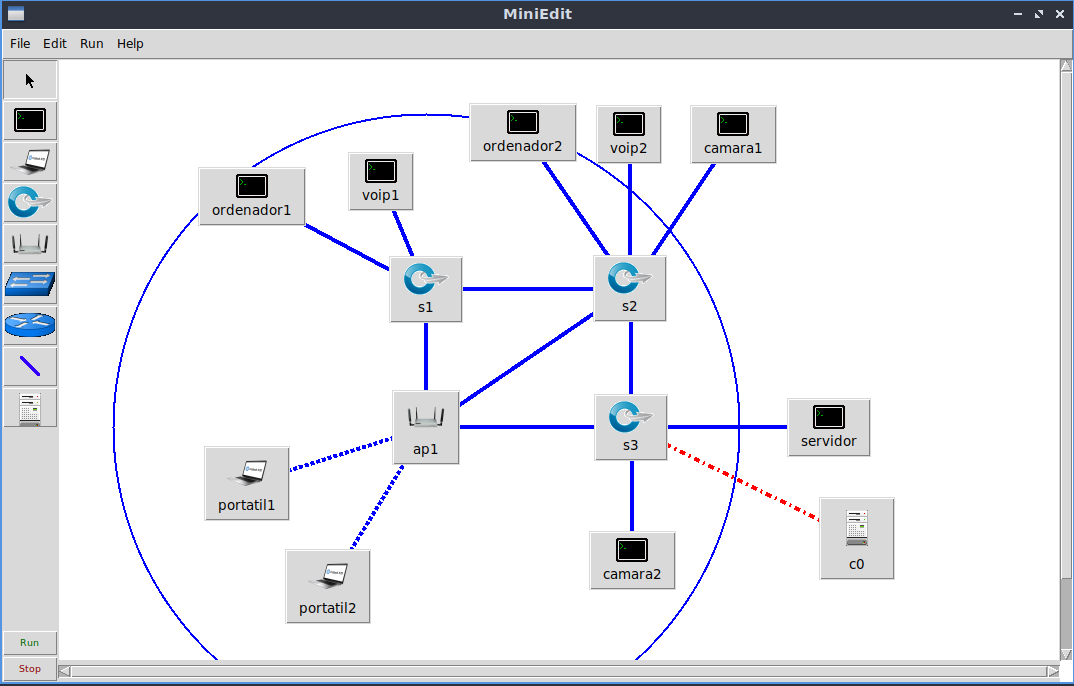
\includegraphics[width=\textwidth]{imagenes/figuras/miniedit.png}
    \caption{Maqueta de la red en la interfaz gráfica de MiniEdit}
    \label{fig:miniedit}
\end{figure}

Ahora podemos exportar el mapa a un archivo ejecutable en una consola para simular nuestra red.

Haciendo unos retoques al archivo exportado tenemos nuestra topología \footnote{Archivo topologia\_oficina.py}, que podemos ejecutar mediante

\lstinline{sudo python topologia_oficina.py}

\subsection{Caracterización de nodos}
En este apartado vamos a caracterizar los tráficos de cada uno de los dispositivos de red, para luego poder simularlos con D-ITG y poder hacer pruebas sobre la capacidad de la red.

\subsubsection{Puestos de trabajo finales}
Los puestos de trabajo están formados por un ordenador de sobremesa. Estos realizarán tareas de compartición de archivos con un servidor central y navegación puntual por internet. No tienen grandes requerimientos de ancho de banda pero si de disponibilidad, para evitar caídas del servicio, sobre todo en horario laboral.

En nuestro entorno de pruebas vamos a utilizar un perfil del generador de tráfico que mantenga un tráfico constante de baja velocidad con picos de hasta 4 Mbps. Este lo hemos extraído de la documentación oficial de la herramienta.\cite{DITG281M63:online}

\lstinline{ITGSend -a <ip_receptor> -T TCP -B E 100 W 4 1000 -o 600}

\subsubsection{Teléfonos IP}
Junto a los ordenadores de sobremesa se encuentra un teléfono IP. Estos están conectados a una red separada de los ordenadores y tienen un bajo requerimiento de ancho de banda pero si son muy sensibles a latencia y jitter en la red, por lo que la red debería ser capaz de proveer algún mecanismo de calidad de servicio para evitar bajadas de calidad en la comunicación.

El generador de tráfico tiene un mecanismo integrado de generación de tráfico que simula una conversación VoIP.

\lstinline{ITGSend -a <ip_receptor> VoIP}

\subsubsection{Dispositivos auxiliares: impresoras en red}
Además se va a instalar una impresora compartida entre todos los ordenadores de la red. Su único requerimiento es estar disponible a los usuarios cuando estos quieran utilizarla.

A la impresora simplemente le vamos a realizar pings, puesto que su carga de red no es significativa en el entorno que estamos estudiando.

\subsubsection{Cámaras de videovigilancia}
En el escenario que estamos planteando se va a incluir una red de videovigilancia. Las cámaras IP habituales tienen unos requisitos medios de ancho de banda ya que envían la señal comprimida al servidor central. Los flujos de vídeo además toleran bien la pérdida de paquetes siempre que esta no sea muy significativa. \cite{boulos:hal-00354947}. Lo realmente importante en este punto es que las cámaras no sean accesibles por ningún otro dispositivo de la red que no sea parte de la subred de seguridad.

Basándonos en una instalación preexistente de seguridad con una cámara IP con una resolución de 1280x720 píxeles hemos determinado que un ancho de banda constante de 70Kbps son suficientes para enviar vídeo al servidor de seguridad. Por esto el tráfico generado será el siguiente:

\lstinline{ITGSend -a <ip_receptor> -T UDP -C 100 -c 70}

\subsubsection{Red wifi: móviles y portátiles}

En el escenario que estamos planteando necesitamos que la red wifi sirva de acceso a los mismos recursos que los ordenadores de sobremesa, puesto que los empleados tienen sus propios dispositivos portátiles de trabajo y deberían ser capaces de usarlos en la oficina. Sus requisitos son exactamente los mismos que los puestos fijos de trabajo.